\clearpage
\setcounter{section}{-1}
\section{What is a metric space?}

\topic{Finding the right method quickly}
\begin{method}{Translate the command into a first line}
\begin{tabular}{p{.32\linewidth}p{.61\linewidth}}
\textbf{Question asks you to}\quad & \textbf{Start with}\rule{0pt}{4ex}\\
Verify a metric & Check finiteness, nonnegativity, zero iff equality, symmetry, then triangle inequality.\\[4pt]
Prove $U$ open & ``Let $p\in U$. Choose $r=\cdots>0$. If $d(x,p)<r$, then $x\in U$.''\\[4pt]
Prove $F$ closed & Take $x_n\in F$ with $x_n\to x$ in the ambient space; prove $x\in F$.\\[4pt]
Find closure/boundary & Classify points by whether every ball meets the set, or both set and complement.\\[4pt]
Prove continuity & Find $\delta$, use convergent sequences, or test inverse images of open sets.\\[4pt]
Prove density & Fix any ball $B_r(p)$ and produce a point of the proposed dense set inside it.\\[4pt]
Prove completeness & Start with an arbitrary Cauchy sequence; construct its limit and keep it inside the space.\\[4pt]
Prove compactness & In $\R^n$, use closed and bounded. In general, extract subsequences or use a known compact image/product.\\[4pt]
Apply Banach & Verify nonempty complete space, self-map, uniform contraction constant $q<1$.\\[4pt]
Disprove a universal claim & Give one example and verify both the hypotheses and the failure of the conclusion.
\end{tabular}
\end{method}
\begin{tip}
A proof is a chain of justified statements, not a list of theorem names. State where each assumption enters. For an ``if and only if'', prove both directions. For limits and compactness, explicitly state that the limit belongs to the required set. A diagram can suggest an answer, but arbitrary metric spaces need an argument using distances.
\end{tip}
\begin{note}{Suggested study order}
First learn metric axioms, balls and sequence definitions. Next learn openness, closedness and continuity. Then study completeness and uniform limits. Finally learn sequential compactness and products. Revisit real analysis whenever a proof uses a supremum, an infimum or a subsequence. After each topic, attempt its question before reading the answer; then reproduce the proof with the answer hidden.
\end{note}


\topic{Metric axioms and core examples}
\begin{note}{What a metric means}
A metric is a function $d:S\times S\to[0,\infty)$ satisfying, for all $x,y,z\in S$,
\[d(x,y)=0\iff x=y,\qquad d(x,y)=d(y,x),\qquad d(x,z)\le d(x,y)+d(y,z).\]
Distances must be finite. A metric space is the pair $(S,d)$: the same set with a different metric may have different convergence, boundedness or completeness properties.

Intuition: distance distinguishes points, is independent of direction, and a detour cannot beat the direct distance. Most metric proofs reduce to the triangle inequality.
\end{note}
\begin{method}{Metric verification}
Check the candidate is defined and finite on every pair. Prove definiteness in both directions. Prove symmetry. For the triangle inequality, either apply a known norm inequality, work pointwise then sum/supremise, or split cases for piecewise formulas. To disprove a candidate it suffices to exhibit one failed axiom. For example $d(x,y)=|x-y|^2$ fails with $x=0,y=1,z=2$, since $4>1+1$.
\end{method}
\begin{note}{Discrete metric and counting metric}
The discrete metric is $d(x,y)=0$ for $x=y$ and $1$ otherwise. It works on \emph{any} set. If $x\ne z$, at least one of $x\ne y$ and $y\ne z$ holds, so the right side of the triangle inequality is at least $1$.

For finite subsets $A,B$ of a set,
\[d(A,B)=\#(A\triangle B),\qquad A\triangle B=(A\setminus B)\cup(B\setminus A).\]
This counts the membership changes needed to transform $A$ into $B$. Since
\[A\triangle C\subseteq(A\triangle B)\cup(B\triangle C),\]
cardinality gives the triangle inequality. If the underlying set is infinite, restrict to finite subsets to ensure the formula stays finite.
\end{note}
\begin{exam}{Section 0 Exercises 0.1 and 0.4: model metric proofs}
(a) Prove the discrete metric is a metric. (b) Prove the counting metric satisfies the triangle inequality.
\end{exam}
\begin{answer}
(a) Its values are $0$ and $1$, hence finite and nonnegative. By definition $d(x,y)=0$ exactly when $x=y$. Equality/inequality of points is symmetric, so $d(x,y)=d(y,x)$. Let $x,y,z\in S$. If $x=z$, the left side is zero, so the triangle inequality holds. If $x\ne z$, $x=y=z$ is impossible, so $d(x,y)+d(y,z)\ge1=d(x,z)$. This proves all axioms.

(b) Let $s\in A\triangle C$. Its membership in $A$ and $C$ differs. If its membership in $B$ agrees with $A$, it differs from $C$, so $s\in B\triangle C$. Otherwise $s\in A\triangle B$. Hence the displayed inclusion holds. For finite sets,
\[\#(A\triangle C)\le\#((A\triangle B)\cup(B\triangle C))\le\#(A\triangle B)+\#(B\triangle C).\]
This is precisely $d(A,C)\le d(A,B)+d(B,C)$.
\end{answer}
\begin{note}{Norm metrics and $\ell^p$ examples}
Every norm gives $d(x,y)=\norm{y-x}$. In $\R^n$ or $\C^n$,
\[\norm{x}_p=\left(\sum_{i=1}^n|x_i|^p\right)^{1/p}\ (1\le p<\infty),\qquad \norm{x}_\infty=\max_i|x_i|.\]
$p=1$ is Manhattan distance, $p=2$ Euclidean distance, $p=\infty$ maximum distance. Their unit spheres in $\R^2$ are respectively a diamond, circle and square. For $1<p<2$ the curve $|x|^p+|y|^p=1$ lies between diamond and circle; for $p>2$ it lies between circle and square.

The inequalities
\[\norm{x}_\infty\le\norm{x}_p\le n^{1/p}\norm{x}_\infty\]
show equivalence of these finite-dimensional norms. For $p=1$ sum scalar triangle inequalities; for $p=\infty$ bound every coordinate by the same maximum bound. The general triangle inequality is Minkowski's inequality (Appendix I).
\end{note}
\begin{exam}{2023 Q2(a): norms, metrics and matrices}
Show that a norm induces a metric and give a norm on $M_2(\R)$ with justification.
\end{exam}
\begin{answer}
Set $d(x,y)=\norm{y-x}$. It is finite and nonnegative. Definiteness gives $d(x,y)=0\iff y-x=0\iff x=y$. Homogeneity with scalar $-1$ gives symmetry. Finally,
\[d(x,z)=\norm{z-x}=\norm{(z-y)+(y-x)}\le\norm{z-y}+\norm{y-x}=d(y,z)+d(x,y).\]
On matrices define $\norm{A}=\sum_{i,j=1}^2|a_{ij}|$. The sum is nonnegative and is zero iff all entries vanish. Also $\norm{\lambda A}=|\lambda|\norm{A}$, and
\[\norm{A+B}=\sum_{i,j}|a_{ij}+b_{ij}|\le\sum_{i,j}|a_{ij}|+\sum_{i,j}|b_{ij}|=\norm{A}+\norm{B}.\]
Thus it is a norm. The Frobenius norm is another valid choice, using the Euclidean norm of the four entries.
\end{answer}
\begin{note}{Visual explanation: unit spheres under different norms}
\begin{center}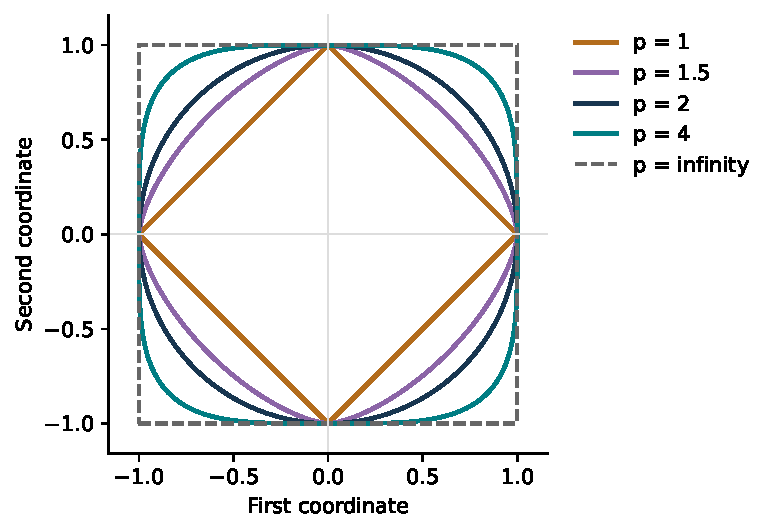
\includegraphics[width=.92\linewidth]{figures/unit_spheres.pdf}\end{center}
Each curve consists of vectors of norm one for a different norm on the same plane. The changing shape is a change of distance rule, not of the underlying points. The unit ball is the region inside its curve; the closed ball also includes the curve. This picture also supports Exercise 3.9.
\end{note}


\topic{Function metrics, Hausdorff distance and unusual metrics}
\begin{note}{Integral and sup metrics on functions}
For continuous real functions on $I=[0,1]$,
\[d_1(f,g)=\int_I|f-g|,\qquad d_{\sup}(f,g)=\sup_{t\in I}|f(t)-g(t)|.\]
The first measures total discrepancy; the second measures worst-case discrepancy. Integral definiteness uses continuity, as proved earlier. For the sup metric, definiteness follows because if the supremum is zero, every pointwise difference is zero. The pointwise inequality
\[|f(t)-h(t)|\le|f(t)-g(t)|+|g(t)-h(t)|\le d_{\sup}(f,g)+d_{\sup}(g,h)\]
gives the triangle inequality upon taking a supremum.

Since $d_1\le d_{\sup}$, uniform convergence implies integral convergence. The converse fails: continuous triangular spikes of height $1$ and support $[0,1/n]$ have integral $1/(2n)$ but sup norm $1$.
\end{note}
\begin{note}{The general sup-metric space $\ell^\infty(S;E)$}
This is the set $F_b(S;E)$ of functions with bounded image, with metric
\[d_{\sup}(f,g)=\sup_{s\in S}d_E(f(s),g(s)).\]
For nonempty $S$, fix $s_0\in S$. Then
\[d(f(s),g(s))\le\diam f(S)+d(f(s_0),g(s_0))+\diam g(S),\]
so the supremum is finite. Metric axioms follow pointwise and then by taking the supremum. For empty $S$ there is a single function; give that singleton its zero metric. No vector-space structure of $E$ is required.
\end{note}
\begin{note}{Hausdorff distance: distance between whole sets}
For nonempty closed bounded subsets of $\R^n$, put
\[d_H(A,B)=\max\left\{\sup_{a\in A}\dist(a,B),\ \sup_{b\in B}\dist(b,A)\right\}.\]
Equivalently, it is the infimum of $\delta\ge0$ such that each set lies in the other's $\delta$-fattening. Nonemptiness makes the distance-to-set expression meaningful; boundedness ensures finiteness; closedness ensures zero distance means equality.

If $A\subseteq B$, then $A_\delta\subseteq B_\delta$. If $x\in(A_\gamma)_\delta$, choose $y\in A_\gamma$ with $d(x,y)\le\delta$ and $a\in A$ with $d(y,a)\le\gamma$. Then $d(x,a)\le\gamma+\delta$, so $(A_\gamma)_\delta\subseteq A_{\gamma+\delta}$ (for the fattenings defined by existence in the supplied notes).
\end{note}
\begin{exam}{Section 0 Exercise 0.6: Hausdorff triangle inequality}
Deduce $d_H(A,C)\le d_H(A,B)+d_H(B,C)$ from the fattening properties.
\end{exam}
\begin{answer}
Let $a=d_H(A,B)$ and $b=d_H(B,C)$, and fix $\varepsilon>0$. By the definition of infimum and monotonicity of fattening, choose admissible radii $r<a+\varepsilon$ and $s<b+\varepsilon$ such that $A\subseteq B_r$, $B\subseteq A_r$, $B\subseteq C_s$, $C\subseteq B_s$. Then
\[A\subseteq B_r\subseteq(C_s)_r\subseteq C_{r+s},\qquad C\subseteq B_s\subseteq(A_r)_s\subseteq A_{r+s}.\]
Thus $d_H(A,C)\le r+s<a+b+2\varepsilon$. Let $\varepsilon\downarrow0$ to obtain the triangle inequality. The small error terms avoid assuming an infimum is attained.
\end{answer}
\begin{note}{TGV metrics and pullbacks}
On $\R^2$, the TGV metric is $d_T(x,y)=\norm{x}_2+\norm{y}_2$ for distinct points and zero on the diagonal. The radial variant uses $\norm{x-y}_2$ when $x,y$ are linearly dependent, and the sum of norms otherwise.

For $d_T$, if the intermediate point equals an endpoint the triangle inequality is equality; otherwise the right side includes the norms of both endpoints and an additional $2\norm{y}$. For the radial variant, distances are lengths of shortest permitted paths along lines through the origin. Algebraically: if the endpoints are dependent, each leg dominates Euclidean distance. If the endpoints are independent and both legs are independent, the result is immediate. If exactly one leg is dependent, use $\norm{x}\le\norm{x-y}+\norm{y}$ (or the analogous inequality for the other endpoint). Both legs cannot be dependent with $y\ne0$ unless the endpoints are dependent. With $y=0$, both legs sum to $\norm{x}+\norm{z}$.

An injective map $\phi:A\to(E,d)$ defines a pullback metric $d_A(x,y)=d(\phi(x),\phi(y))$. Injectivity is needed for definiteness. Example:
\[d_{NS}(x,y)=|\arctan x-\arctan y|\quad(x,y\in\R).\]
This is bounded by $\pi$ and is isometric to the usual interval $(-\pi/2,\pi/2)$. It is not induced by a norm on $\R$, because a norm would make $d(0,n)=n\norm{1}$ unbounded.
\end{note}
\begin{exam}{Additional practice: why continuity depends on the metric}
For the TGV metric on $\R$, show that the identity from TGV to the usual metric is Lipschitz, but the reverse identity is continuous only at zero.
\end{exam}
\begin{answer}
For distinct $x,y$, $|x-y|\le|x|+|y|=d_T(x,y)$; on the diagonal both distances are zero. Thus the identity to the usual metric is $1$-Lipschitz. At zero $d_T(x,0)=|x|$, so the reverse identity is continuous there. If $a\ne0$, take $x_n=a+1/n$. Then $x_n\to a$ in the usual metric but $d_T(x_n,a)=|a+1/n|+|a|\to2|a|>0$. Therefore the reverse identity is not continuous at $a$ and the metrics are not topologically equivalent.
\end{answer}


\topic{Proof clinic: Quantifiers: what the examiner is asking you to construct}
\begin{note}{Read a definition as a conversation}
For openness, someone gives you a point $p\in U$. You must answer with a positive radius $r$, and then prove that \emph{every} point inside that ball stays in $U$. Your radius may depend on $p$. This is why an interval such as $(0,1)$ is open even though points near its endpoints need very small radii.

For convergence, someone gives you an accuracy $\varepsilon>0$. You must answer with a cutoff $N$, after which \emph{every} term is close enough. A finite number of failures before $N$ does not matter. The cutoff may depend on $\varepsilon$, but not on the later index $n$.

For Cauchyness, after your cutoff all pairs of terms must be close. You do not choose a separate cutoff for each later pair. That is why showing $d(x_n,x_{n+1})\to0$ does not suffice: it controls adjacent terms, rather than arbitrary pairs.

For sequential compactness, you are given any sequence and must extract a suitable subsequence. You do not need the original sequence itself to converge. For example $(-1)^n$ lies in the compact interval $[-1,1]$ but does not converge; its even subsequence is constantly $1$.
\end{note}
\begin{exam}{Additional practice: spot the quantifier error}
A student argues: ``For each $n$, choose $N=n+1$. Then all terms after $N$ are late, so the sequence converges.'' What is missing?
\end{exam}
\begin{answer}
There is no proposed limit and no bound on the distance to it. More fundamentally, the required cutoff must be chosen after the tolerance but before the universally quantified later index. Writing $N=n+1$ makes the cutoff depend on the very index it is supposed to control. A valid proof must name a point $a$ and, for each $\varepsilon$, choose one $N(\varepsilon)$ such that $d(x_n,a)<\varepsilon$ holds for every $n\ge N(\varepsilon)$.
\end{answer}


\topic{Proof clinic: A manageable routine for each topic}
\begin{note}{Use the expanded notes actively}
\textbf{First pass:} read the intuitive explanation and one example. Say the idea aloud in ordinary words. For instance, complete means that sequences whose terms become mutually close do not run into missing points.

\textbf{Second pass:} write the formal definition from memory. Check every quantifier and where the metric is evaluated. Then reconstruct the proof's main estimate before reading the intermediate steps.

\textbf{Third pass:} attempt a numbered lecture exercise. Read only the method box if stuck. After checking the solution, close the notes and write the argument again in your own words.

\textbf{Fourth pass:} attempt a past-paper question on the same topic. Give reasons for each implication and verify every theorem hypothesis. Collect an example and a counterexample beside the definition.

The objective is to recognise the structure of a new question: local-radius construction, sequence-limit argument, infimum approximation, uniform-error estimate, subsequence extraction, or fixed-point verification. Those structures recur across the whole supplied module material.
\end{note}


\topic{Worked lecture exercises}
\begin{note}{How to read this workbook}
Each exercise starts with the task, then gives the reason for the chosen method, a complete solution and a reusable lesson. The statements are restated in a compact form; consult the original exercise sheet for the original wording. Try the question first. If stuck, read the method box, cover the solution, and try again.
\end{note}
\exercise{0.1}{The discrete metric}
\begin{exam}{Lecture exercise}
For any set $S$, put $d(x,y)=0$ if $x=y$ and $d(x,y)=1$ otherwise. Prove $d$ is a metric.
\end{exam}
\begin{method}{Use the two possible values}
The first axioms follow directly from the definition. The triangle inequality only needs thought when its left side is $1$. Ask whether both terms on the right could then be zero.
\end{method}
\begin{answer}
The function is defined for every pair and takes finite nonnegative values. By construction, $d(x,y)=0$ exactly when $x=y$. Since $x=y$ iff $y=x$, the definition gives $d(x,y)=d(y,x)$.

Fix $x,y,z\in S$. If $x=z$, then $d(x,z)=0$ and the right side of the triangle inequality is nonnegative. If $x\ne z$, then at least one of $x\ne y$, $y\ne z$ holds: otherwise $x=y=z$, a contradiction. Therefore at least one of $d(x,y),d(y,z)$ is $1$, giving
\[d(x,z)=1\le d(x,y)+d(y,z).\]
Thus the triangle inequality holds for every triple, and $d$ is a metric.
\end{answer}
\begin{tip}
Do not assume the three points are distinct. A metric axiom must hold for repeated points too. Separating the case $x=z$ handles this safely.
\end{tip}
\exercise{0.2}{Why integral distance distinguishes continuous functions}
\begin{exam}{Lecture exercise}
For continuous $h:[0,1]\to\R$, prove $\int_0^1|h(t)|\,dt=0\Rightarrow h=0$.
\end{exam}
\begin{method}{Prove the contrapositive}
If $h$ is nonzero somewhere, continuity prevents its absolute value from dropping immediately to zero. It stays above a positive height on an interval of positive length; that creates positive area.
\end{method}
\begin{answer}
Suppose $h\ne0$. Then $h(p)\ne0$ for some $p\in[0,1]$. Let $c=|h(p)|>0$. By continuity there is $\delta>0$ such that
\[t\in[0,1],\ |t-p|<\delta\quad\Rightarrow\quad |h(t)-h(p)|<c/2.\]
The reverse triangle inequality gives
\[|h(t)|\ge |h(p)|-|h(t)-h(p)|>c/2.\]
The relative neighbourhood $[0,1]\cap(p-\delta,p+\delta)$ contains a closed interval $J$ of positive length, including when $p$ is an endpoint. Since $|h|\ge0$ everywhere,
\[\int_0^1|h|\ge\int_J|h|\ge(c/2)|J|>0.\]
Thus nonzero $h$ forces positive integral. Its contrapositive is the requested implication. Applied to $h=f-g$, it proves definiteness of $d_1$ on continuous functions.
\end{answer}
\begin{tip}
The integrand being nonnegative is not enough for pointwise vanishing: a function supported at one point has zero integral. Continuity supplies the interval on which the positive lower bound holds.
\end{tip}
\exercise{0.3}{The sup metric}
\begin{exam}{Lecture exercise}
For $f,g\in C([0,1];\R)$, let $d_{\sup}(f,g)=\sup_t|f(t)-g(t)|$. Prove definiteness and triangle inequality.
\end{exam}
\begin{answer}
Continuous functions on the compact interval are bounded, so the supremum is finite. If $d_{\sup}(f,g)=0$, then for every $t$,
\[0\le |f(t)-g(t)|\le d_{\sup}(f,g)=0.\]
Therefore $f(t)=g(t)$ for every $t$, so $f=g$. Conversely $f=g$ makes every difference zero, giving $d_{\sup}(f,g)=0$.

For any continuous $h$ and any fixed $t$,
\begin{align*}
|f(t)-h(t)|&\le |f(t)-g(t)|+|g(t)-h(t)|\\
&\le d_{\sup}(f,g)+d_{\sup}(g,h).
\end{align*}
The last bound does not depend on $t$. It is therefore an upper bound for all the numbers whose supremum defines $d_{\sup}(f,h)$. Consequently
\[d_{\sup}(f,h)\le d_{\sup}(f,g)+d_{\sup}(g,h).\]
\end{answer}
\begin{method}{The transferable step}
First bound every pointwise expression by a common constant; then take the supremum. A supremum is a least upper bound, so it is at most any upper bound you have proved.
\end{method}
\exercise{0.4}{Counting distance}
\begin{exam}{Lecture exercise}
For finite sets $A,B$, let $d(A,B)=\#(A\triangle B)$. Prove the triangle inequality.
\end{exam}
\begin{answer}
Fix a third finite set $C$. We prove
\[A\triangle C\subseteq(A\triangle B)\cup(B\triangle C).\]
Take $s\in A\triangle C$. If $s\in A$ and $s\notin C$, either $s\in B$, giving $s\in B\setminus C$, or $s\notin B$, giving $s\in A\setminus B$. If instead $s\in C$ and $s\notin A$, either $s\in B$, giving $s\in B\setminus A$, or $s\notin B$, giving $s\in C\setminus B$. In every case $s$ belongs to the union on the right.

Cardinality is monotone under inclusion, and the size of a finite union is at most the sum of the sizes. Hence
\begin{align*}
d(A,C)&=\#(A\triangle C)\\
&\le\#((A\triangle B)\cup(B\triangle C))\\
&\le\#(A\triangle B)+\#(B\triangle C)=d(A,B)+d(B,C).
\end{align*}
\end{answer}
\begin{note}{A concrete check}
For $A=\{1,2\}$, $B=\{2,3\}$ and $C=\{3,4\}$, the three distances are $2,2,4$, so the triangle inequality is equality. The proof must work for all sets, but a numerical example helps check the interpretation.
\end{note}
\exercise{0.5}{TGV and radial TGV triangle inequalities}
\begin{exam}{Lecture exercise}
Write $\norm{\cdot}=\norm{\cdot}_2$. On $\R^2$ define
\[d_T(x,z)=\begin{cases}0,&x=z,\\\norm{x}+\norm{z},&x\ne z,\end{cases}\]
and define $d_R(x,z)=\norm{x-z}$ when $x,z$ are linearly dependent, and $\norm{x}+\norm{z}$ otherwise. Prove the triangle inequality for both.
\end{exam}
\begin{method}{Split by the formula for the left side}
For the radial metric, dependent endpoints use Euclidean triangle inequality. For independent endpoints, study whether each leg of the detour is dependent. The zero intermediate point needs its own sentence.
\end{method}
\begin{answer}
For $d_T$, fix $x,y,z$. If $x=z$, the left side is zero. If $y=x$ or $y=z$, the inequality is equality. In the remaining case $x\ne z$ and $y$ is different from both, so
\[d_T(x,y)+d_T(y,z)=\norm{x}+2\norm{y}+\norm{z}\ge\norm{x}+\norm{z}=d_T(x,z).\]

For $d_R$, first note that $d_R(u,v)\ge\norm{u-v}$ in every case, by the Euclidean triangle inequality.

If $x,z$ are dependent, then
\[d_R(x,z)=\norm{x-z}\le\norm{x-y}+\norm{y-z}\le d_R(x,y)+d_R(y,z).\]
Now suppose $x,z$ are independent. Then $d_R(x,z)=\norm{x}+\norm{z}$. If $y=0$, the two legs have sum $\norm{x}+\norm{z}$, so the result holds. Assume $y\ne0$.

If both pairs $(x,y)$ and $(y,z)$ are independent, their distances sum to $\norm{x}+2\norm{y}+\norm{z}$, which is large enough. If $x,y$ are dependent and $y,z$ independent, then
\[d_R(x,y)+d_R(y,z)=\norm{x-y}+\norm{y}+\norm{z}\ge\norm{x}+\norm{z}.\]
If $x,y$ are independent and $y,z$ dependent, use $\norm{z}\le\norm{z-y}+\norm{y}$ instead. Finally both pairs cannot be dependent when $y\ne0$: each endpoint would be a scalar multiple of $y$, making $x,z$ dependent. These cases exhaust all possibilities.
\end{answer}
\begin{tip}
The metric is piecewise defined, so ``by triangle inequality'' alone hides the main difficulty. State which branch applies and which Euclidean inequality justifies that branch.
\end{tip}
\exercise{0.6}{Fattenings and Hausdorff triangle inequality}
\begin{exam}{Lecture exercise}
For $A_\delta=\{x:\exists a\in A,\ \norm{x-a}_2\le\delta\}$, prove monotonicity in $A$, prove $(A_\gamma)_\delta\subseteq A_{\gamma+\delta}$, then deduce the Hausdorff triangle inequality.
\end{exam}
\begin{answer}
If $A\subseteq B$ and $x\in A_\delta$, a witness $a\in A$ to $\norm{x-a}\le\delta$ also belongs to $B$. Hence $x\in B_\delta$, proving $A_\delta\subseteq B_\delta$.

If $x\in(A_\gamma)_\delta$, choose $y\in A_\gamma$ with $\norm{x-y}\le\delta$, then $a\in A$ with $\norm{y-a}\le\gamma$. Thus $\norm{x-a}\le\norm{x-y}+\norm{y-a}\le\delta+\gamma$, so $x\in A_{\gamma+\delta}$.

Let $A,B,C$ be nonempty closed bounded Euclidean sets and let $h=d_H(A,B)$, $k=d_H(B,C)$. Fix $\varepsilon>0$. Choose admissible radii $r<h+\varepsilon$ and $s<k+\varepsilon$. This means $A\subseteq B_r$, $B\subseteq A_r$, $B\subseteq C_s$ and $C\subseteq B_s$. Then
\[A\subseteq B_r\subseteq(C_s)_r\subseteq C_{r+s},\qquad C\subseteq B_s\subseteq(A_r)_s\subseteq A_{r+s}.\]
Therefore $r+s$ is an admissible radius between $A,C$, giving
\[d_H(A,C)\le r+s<h+k+2\varepsilon.\]
Letting $\varepsilon\downarrow0$ proves $d_H(A,C)\le d_H(A,B)+d_H(B,C)$.
\end{answer}
\begin{tip}
The set inclusion is one-sided; equality is unnecessary. The $\varepsilon$ terms avoid assuming that the infimum in the Hausdorff definition has an admissible minimising radius.
\end{tip}
